\section{Kết quả và thảo luận}
\label{sec:results}

\subsection{Bảng kết quả tổng quan}

Bảng~\ref{tab:overall-results} tổng hợp kết quả trung bình trên 15 màn chơi.
Mỗi thuật toán được chạy ba lần trên từng màn chơi.

\begin{table}[H]
\centering
\caption{Kết quả thực nghiệm trung bình trên 15 màn chơi}
\label{tab:overall-results}
\small
\setlength{\tabcolsep}{4pt}
\begin{tabular}{@{}lrrrrrr@{}}
\toprule
\multirow{2}{*}{\textbf{Thuật toán}} &
\multicolumn{3}{c}{\textbf{Hiệu năng tìm kiếm}} &
\multicolumn{3}{c}{\textbf{Lời giải}} \\
\cmidrule(lr){2-4}\cmidrule(l){5-7}
& \textbf{Thời gian (ms)} & \textbf{Bộ nhớ (KiB)} & \textbf{Nút}
& \textbf{Độ dài} & \textbf{Thao tác} & \textbf{Chi phí} \\
\midrule
BFS & 68,35 & 174,31 & 619,73 & 15,40 & 16,00 & 16,00 \\
DFS & 49,74 & 143,96 & 438,20 & 125,20 & 139,87 & 139,87 \\
UCS & 89,54 & 174,00 & 671,33 & 15,40 & 16,00 & 16,00 \\
A*  & 52,25 & 120,87 & 350,60 & 15,40 & 16,07 & 16,00 \\
\bottomrule
\end{tabular}
\end{table}

Trong bảng, \emph{Độ dài} chỉ đếm các bước di chuyển, còn \emph{Thao tác}
tính cả \textsc{SwitchCube}. Cột \emph{Chi phí} của BFS/DFS là số hành động
đơn vị; UCS/A* dùng hàm chi phí 0/1/2 ở Bảng~\ref{tab:cost}. Vì vậy, cột này
chỉ cho phép so sánh trực tiếp UCS với A*. Khi đánh giá lại đường BFS bằng cùng
hàm chi phí 0/1/2 của UCS, cả 15 màn chơi đều cho chi phí bằng đường UCS. Bộ
màn chơi này chưa có trường hợp UCS chọn đường rẻ hơn BFS; hai thuật toán khác
nhau chủ yếu ở cách duyệt và số nút mở rộng.

\subsection{Biểu đồ theo màn chơi}

Ba biểu đồ ở Hình~\ref{fig:benchmark-charts} và
Hình~\ref{fig:benchmark-nodes} được tạo từ cùng bộ CSV bằng
Matplotlib~\cite{matplotlib311}. Số liệu từng màn chơi và độ lệch chuẩn thời gian
được lưu trong tệp \texttt{data/benchmark\_summary.csv} đi kèm báo cáo.

\begin{figure}[!tbp]
\centering
\begin{subfigure}[b]{0.96\textwidth}
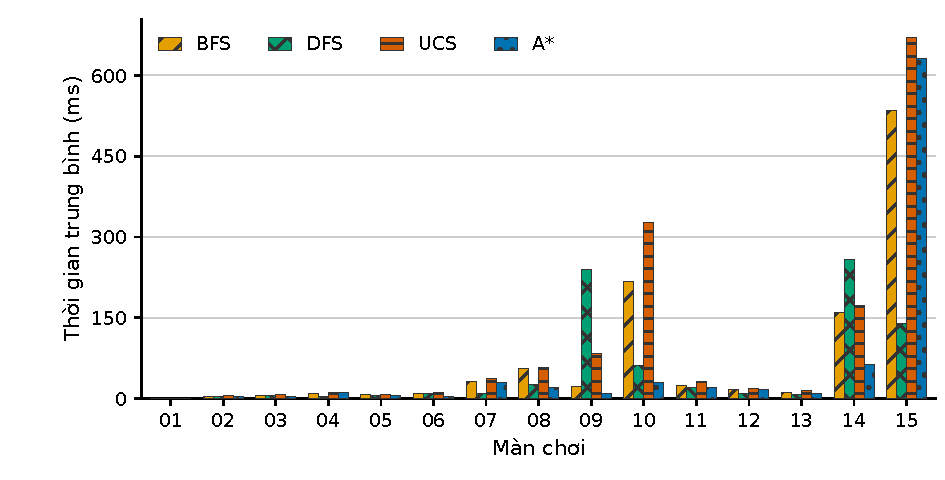
\includegraphics[width=\linewidth]{search_time_ms_readable.pdf}
\caption{Thời gian tìm kiếm trung bình}
\end{subfigure}

\vspace{0.5cm}
\begin{subfigure}[b]{0.96\textwidth}
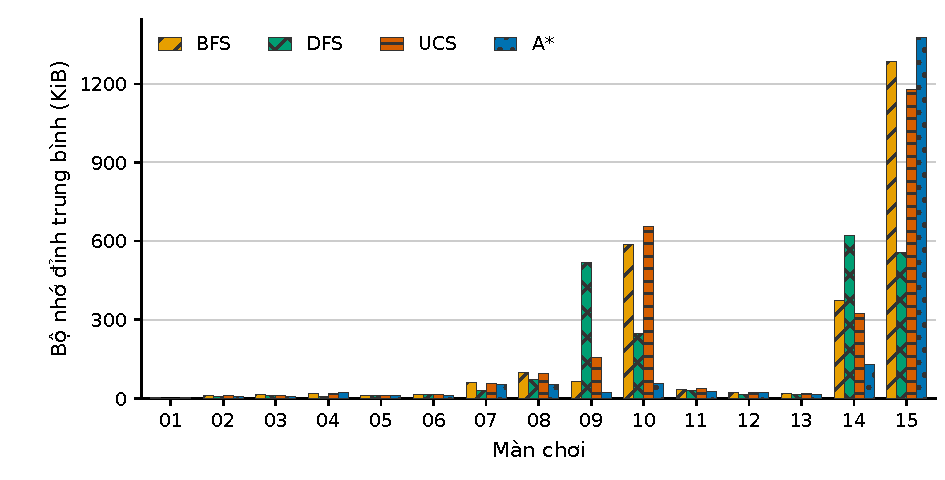
\includegraphics[width=\linewidth]{peak_python_memory_kib_readable.pdf}
\caption{Bộ nhớ Python được theo dõi, tính bằng KiB}
\end{subfigure}
\caption{Thời gian và bộ nhớ theo màn chơi và thuật toán}
\label{fig:benchmark-charts}
\end{figure}

\begin{figure}[!tbp]
\centering
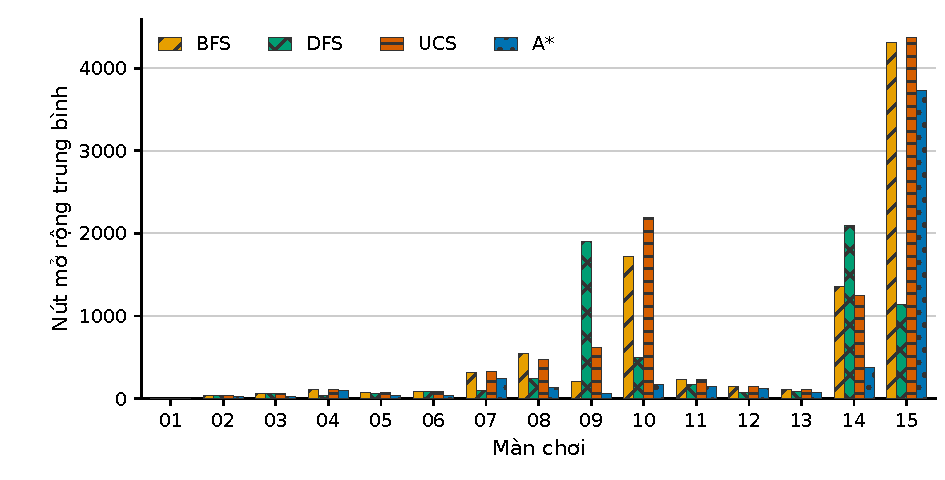
\includegraphics[width=0.96\textwidth]{expanded_nodes_readable.pdf}
\caption{Số nút mở rộng theo màn chơi và thuật toán}
\label{fig:benchmark-nodes}
\end{figure}

\subsection{Chất lượng lời giải và đánh đổi}

DFS có thời gian trung bình thấp nhất, 49,74 ms, nhưng lời giải dài trung bình
125,20 bước; ở màn chơi 15 con số này lên tới 724 bước. Vì thế, tốc độ của DFS
phụ thuộc mạnh vào thứ tự sinh trạng thái kế tiếp và không chứng tỏ chất lượng
lời giải. BFS cho lời giải ít hành động, nhưng tập chờ xét rộng và không xét
chi phí của ô Fragile.

UCS tối ưu theo hàm chi phí 0/1/2 nhưng mở rộng trung bình 671,33 nút và có
thời gian trung bình cao nhất trong bốn thuật toán do không có thông tin hướng
đích. A* đạt cùng chi phí với UCS trên cả 15 màn chơi, đồng thời chỉ mở rộng
trung bình 350,60 nút: thấp hơn BFS 43,4\% và UCS 47,8\%. Tại màn chơi 10,
A* mở rộng 168 nút, so với 1.725 của BFS và 2.191 của UCS.

Số nút mở rộng ít hơn không bảo đảm thời gian thấp hơn. Ở màn chơi 15, A* mất
577,35 ms trong khi BFS mất 488,68 ms; thời gian tính heuristic và quản lý hàng
đợi ưu tiên có thể lớn hơn phần thời gian tiết kiệm nhờ mở rộng ít nút. Trên bộ
15 màn chơi này, A* đạt sự cân bằng tốt giữa chất lượng lời giải, số nút mở rộng
và bộ nhớ. UCS là mốc đối chiếu về chi phí tối ưu; BFS đơn giản nhưng dùng nhiều
bộ nhớ cho tập chờ xét; DFS nhanh ở một số màn chơi nhưng chất lượng lời giải
không ổn định.

Các nhận xét này chỉ dựa trên 15 màn chơi do nhóm xây dựng và ba lần lặp. Bộ
nhớ đỉnh là lượng cấp phát do \texttt{tracemalloc} theo dõi, không phải tổng
RAM của tiến trình; thời gian ở màn chơi nhỏ cũng có thể chịu nhiễu hệ điều
hành.
